\chapter{Código C}
Para servir como ponto de partida e de comparação com os resultados obtidos quando utilizado o GPU foi desenvolvido este código em C com base no exemplo dado no enunciado.

\lstinputlisting[frame=single]{main.c}

Este código executa o algoritmo e calcula e imprime para o terminal o tempo que demora a fazê-lo, e em seguida imprime os dados para um ficheiro de saída.

Um gráfico exemplificativo do funcionamento deste código apresenta-se a seguir, o código foi executado na máquina Diana que nos foi disponibilizada e onde demorou um tempo mediano de 5,7345560 segundos quando N igual a 10000. Apenas foi contabilizado o tempo de execução do algoritmo em si tendo sido ignorado o tempo de alocação de recursos e inicialização destes. 

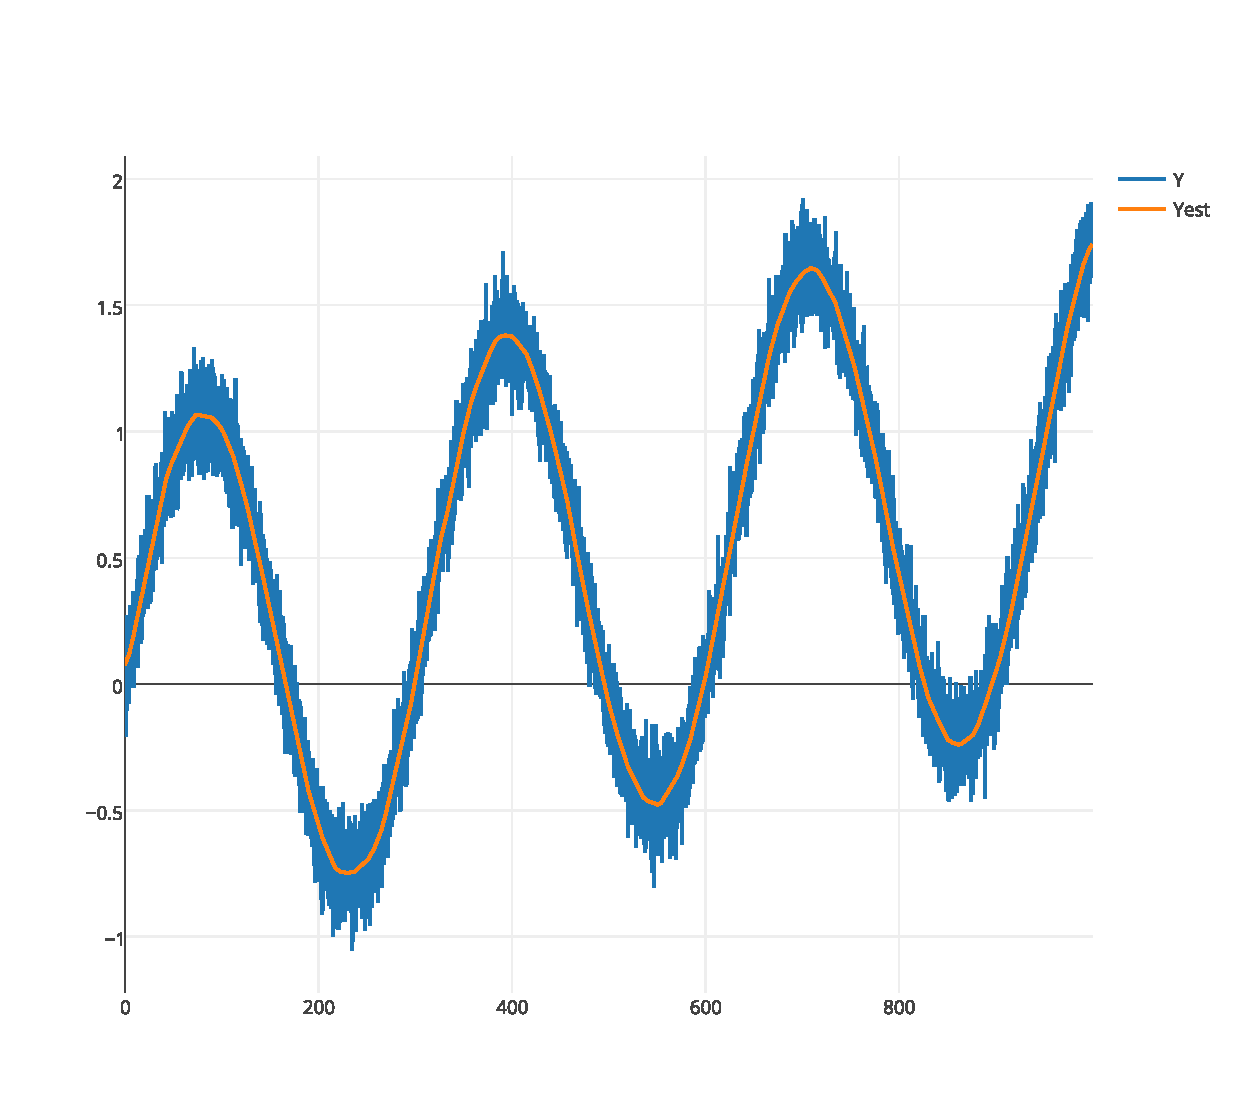
\includegraphics[width=\textwidth]{output}